\documentclass[conference]{IEEEtran}
\usepackage[T1]{fontenc}
\usepackage{times}
\usepackage{amsmath,amssymb}
\usepackage{graphicx}
\usepackage{booktabs}
\usepackage[numbers,sort&compress]{natbib}
\usepackage[hidelinks]{hyperref}
\hypersetup{pdftitle={When Is Robot Recovery Justified? Decision-Sufficient Explanations and the Limits of Observation},pdfauthor={},pdfsubject={Anonymous Stage 1 research paper},pdfkeywords={}}
\newcommand{\Good}{\operatorname{Good}}
\newcommand{\supp}{\operatorname{supp}}
\title{When Is Robot Recovery Justified?\\Decision-Sufficient Explanations and the Limits of Observation}
\author{Anonymous Authors}
\begin{document}
\maketitle
\begin{abstract}
A recovery skill can succeed while available observations cannot justify choosing it. We study the smallest observable evidence sufficient to support a fixed intervention relative to measured paired outcomes. Decision-Sufficient Recovery Explanations (DSRE) return a minimum pure conjunction or witnesses of observational conflict, an inadequate action repertoire, and insufficient reference evidence. The reasoning is ordinary exact rule enumeration, equivalent to strong outcome-aware baselines; our contribution is an intervention-grounded methodology and its measured limits. On 844 qualified simulated checkpoints, one extra Boolean pose predicate raises PickCube finite-reference actionable mass from 183 to 235 of 422. Reused grouped cross-fitting increases successful strict recommendations from 202 to 242, but unacceptable choices from one to two; failed-start successes fall from 19 to 18. A frozen prospective study completed 33 seed parents per task before a runtime interruption. PickCube successful recommendations increase from 29 to 38 of 66 ($+13.64$ percentage points, paired 95\% interval $[6.06,21.21]$), entirely on already-successful starts. A strict depth-2 tree matches these decisions; failed-start successes remain 6/20. PushCube strict coverage stays zero despite 66/66 successful recoveries. This incomplete fresh cohort strengthens the observation/justification distinction, without establishing improved failure recovery, algorithmic superiority, or deployment calibration.
\end{abstract}

\section{Introduction}
A robot must decide whether to continue an ongoing manipulation or invoke a recovery skill. Explaining why a policy predicts ``recover'' is different from showing that recovery is adequate for states consistent with what the robot observed. A high average recovery success rate also need not justify every individual decision: a few indistinguishable states in which the action fails can defeat a universal justification. Conversely, acquiring more detailed observations cannot make an inadequate skill succeed.

We ask: \emph{When is a recovery intervention justified by a minimal set of actually observable facts, and what prevents justification when those facts are insufficient?} Our unit of evidence is a checkpoint with two measured terminal outcomes, one for each fixed continuation. We separate successful completion from improvement over the alternative, and separate descriptive finite-reference claims from guarantees for future deployment. The objective is to characterize justification under an explicit observation vocabulary and action repertoire, rather than to invent a detector or improve the controller.

DSRE supplies three linked outputs: a smallest sufficient observable conjunction, checkable counterexamples when justification fails, and a development-time frontier over a finite menu of observation refinements. A successful conjunction is an exact pure outcome-aware rule. We make this equivalence explicit: an exhaustive baseline with the same grammar, support and ties must produce the same answer. The scientific question concerns what this common semantics reveals about robot interventions, including where apparent gains disappear under stronger controls.

Our study combines exact finite-table analysis with grouped cross-fitting on two fixed simulated tasks. The positive finding is a representation-dependent increase in PickCube justification coverage. The adverse findings are equally central: most gains maintain existing success rather than recover from failure; held-out errors persist; ordinary short rules reproduce major settings; and the entire observation menu fails to justify PushCube decisions despite a strong recovery skill. A fresh, frozen-reference confirmation study tests whether the one-predicate gain persists on previously unused seed parents. Its results will update the claims rather than select a new operating point.

\section{Related Work and Scope of the Contribution}
Minimal sufficient explanations for factored MDPs already justify decisions using reward and occupancy structure~\cite{khan2009}. Anchors target high conditional precision for a predictor under a perturbation distribution~\cite{anchors}; probabilistic sufficient explanations likewise concern preservation of model decisions~\cite{pse}. DSRE instead labels reference states with measured adequacy of two interventions. This changes the target of explanation, not the established idea of sufficient evidence.

Outcome-aware subgroup rules are also established. DISCRET synthesizes rules for treatment-effect estimation~\cite{discret}; our exact risk-aware rule comparator shares the principle of matching observable subgroups to outcomes, without purporting to reproduce its learned synthesis. More fundamentally, robust action intersection under partial observability already covers our strict feasibility criterion~\cite{partial}. Our refinement proposition is an elementary specialization of that principle. We claim no new theorem of partial observability, hitting-set optimization, pure-rule enumeration, or calibration.

Robot recovery research includes corrective actions from violated preconditions in CAPE~\cite{cape} and decision-tree monitoring with recovery under decision uncertainty~\cite{peddi}. Explicit observation of decision context is developed by Ernst et al.~\cite{ernst}. DA-GRD studies grasp-relevant ambiguity reduction through physical sensing~\cite{dagrd}, whereas our optional channels are fixed Boolean summaries of already available simulated poses. RESCUE evaluates alarms through matched counterfactual interventions~\cite{rescue}; we do not claim to introduce intervention-relative evaluation or state branching. The latter two works are cited as preprints. Our narrower contribution is an executable, intervention-grounded sufficiency analysis with distinct obstruction witnesses, equal-information controls, and a measured characterization of its limits. Whether that integrated characterization warrants a robotics contribution remains an empirical and scientific judgment, not an algorithmic superiority claim.

\section{Decision-Sufficient Recovery Evidence}
\subsection{Reference model and observable inputs}
Let $s$ be a full robot--environment state and $x=F(s)$ its predecision observation signature, possibly including a timestamped earlier observation. The fixed actions are $\mathcal A=\{c,r\}$: continue and recover. Executing skill $a$ for the declared horizon gives terminal binary utility $U(s,a)$. The measured reference $R$ contains paired outcomes and independent parent identifiers. Define
\begin{equation}
\Good(s)=\{a\in\mathcal A:U(s,a)=1\}.
\end{equation}
Adequacy is $a\in\Good(s)$, not positive treatment effect. Both actions may be adequate; neither may be. Choosing continue from an already successful state can maintain success, but cannot be counted as a newly recovered failure. Regret relative to the best available action differs from inadequacy: a neither-success state has no successful alternative but still makes a chosen action unacceptable under our adequacy definition.

For known literals $E\subseteq x$, let $M_R(E,x)$ contain all reference rows not contradicted by $E$. An UNKNOWN reference predicate remains compatible; an unknown query value cannot be asserted as a literal. A strict finite-reference justification is $(E,a)$ satisfying
\begin{equation}
\begin{gathered}
|\{\text{parent}(s):s\in M_R(E,x)\}|\ge2,\\
a\in\bigcap_{s\in M_R(E,x)}\Good(s).
\end{gathered}
\label{eq:strict}
\end{equation}
Missing or unqualified outcomes prevent a certificate. The task, skills, horizon, observation map and outcome definition must match the reference scope. Nonempty support prevents vacuous justification, while two independent parents are an explicit reference-support requirement, not a statistical confidence guarantee.

DSRE searches all subsets of known literals for minimum $|E|$. Canonical ties prefer larger row support, then continue, then lexicographic facts. A necessary-literal witness is a compatible row that makes the selected action inadequate when that literal is removed. Minimum cardinality guarantees such a counterexample under the fixed support rule: removing a literal expands support and cannot reduce its parent count. The certificate records scope, matched rows, measured outcomes and reference identity. It says nothing universal about unobserved states.

\begin{figure*}[t]
\centering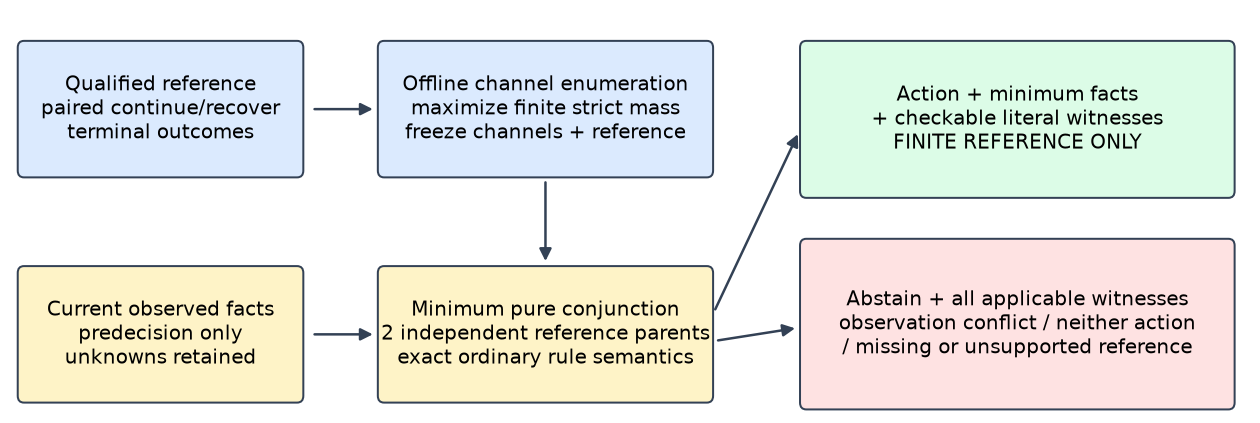
\includegraphics[width=\textwidth]{figures/method.png}
\caption{DSRE separates development-time observation design from query-time justification. Paired intervention outcomes label only the reference; the query sees predecision facts. An action is a finite-reference recommendation, never an automatically calibrated execution permission. All obstruction types can coexist.}
\label{fig:method}
\end{figure*}

\subsection{Why justification fails}
After strict search abstains, DSRE returns all applicable scoped obstructions. \emph{Repertoire inadequacy}: a compatible qualified state has $\Good=\varnothing$. \emph{Observational ambiguity}: compatible states have disjoint nonempty adequate-action sets; with two actions, a continue-only and a recover-only state suffice. \emph{Reference insufficiency}: support is too small, outcomes are missing/unqualified, or scope is inconsistent. A support shortage is not proof of physical impossibility. Why-not witnesses show a failing compatible reference row for each candidate action; they do not assert that the current unknown state is that row.

For example, two PickCube checkpoints share all six primary predicates. At one, object.x$=-.04661$ m and goal.x$=-.01260$ m; continue fails and recover succeeds. At the other, object.x$=.03920$ m and goal.x$=-.01540$ m; neither succeeds. The extra predicate object.x$-$goal.x$<-.02$ separates them and gives the first a pure recovery child supported by two parents in the full reference. It leaves the second inadequate. Such small support is fragile when parents are held out. In PushCube, a recover-only and a continue-only checkpoint share all twelve declared predicates despite different raw poses. No channel in this menu separates them. This is a vocabulary limitation, not an impossibility claim for arbitrary sensors or raw-coordinate reasoning.

\subsection{Observation refinement and known equivalence}
For complete observed signatures, partition $R$ into classes $Z$ and define the descriptive finite ceiling
\begin{equation}
 C_R(F)=\frac1{|R|}\sum_Z |Z|\,mathbf1\!\left[\bigcap_{s\in Z}\Good(s)\ne\varnothing\right].
\end{equation}
This exact-signature ceiling is distinct from supported conservative-rule coverage, particularly with UNKNOWN values. It is also distinct from performance on held-out states evaluated against a smaller training reference.

\noindent\textbf{Proposition (finite refinement).} For deterministic complete predicates on the same fixed reference, if $F'$ refines $F$, then $C_R(F')\ge C_R(F)$. Any neither-success row remains unjustifiable after arbitrary refinement.\newline
\emph{Proof.} Every child of an actionable class retains its common adequate action. A class containing a neither-success row has empty intersection for that row's child. Summing child masses proves the first statement; empty $\Good$ proves the second. $\square$

For $m=6$ optional unit-cost predicates, enumerate $J$ with $|J|\le b$, maximize training $C_R(F_0\cup J)$, then minimize cost and use canonical channel ties. This is offline instrumentation design, not online active sensing. The budget counts predicates, not physical sensors, latency or energy. With $d$ known query facts and $n$ reference rows, direct strict search costs $O(n d2^d)$ and memory can be bounded by cached bit masks. Channel selection considers at most $2^m$ menus. These small exact searches are practical here, without implying scalability to arbitrary vocabularies.

B7, exhaustive zero-error outcome-aware rules with identical support and ties, is mathematically identical to DSRE. Two-literal rules are a restricted grammar; risk-aware B5 allows empirical error at most $.1$ and is provisional, not strict. An exact rule's name or witness format does not constitute an algorithmic advantage. Adding predicates preserves old rules on a fixed table, but neither cross-fit performance nor a selector choosing nonnested menus must improve monotonically.

\begin{figure*}[t]
\centering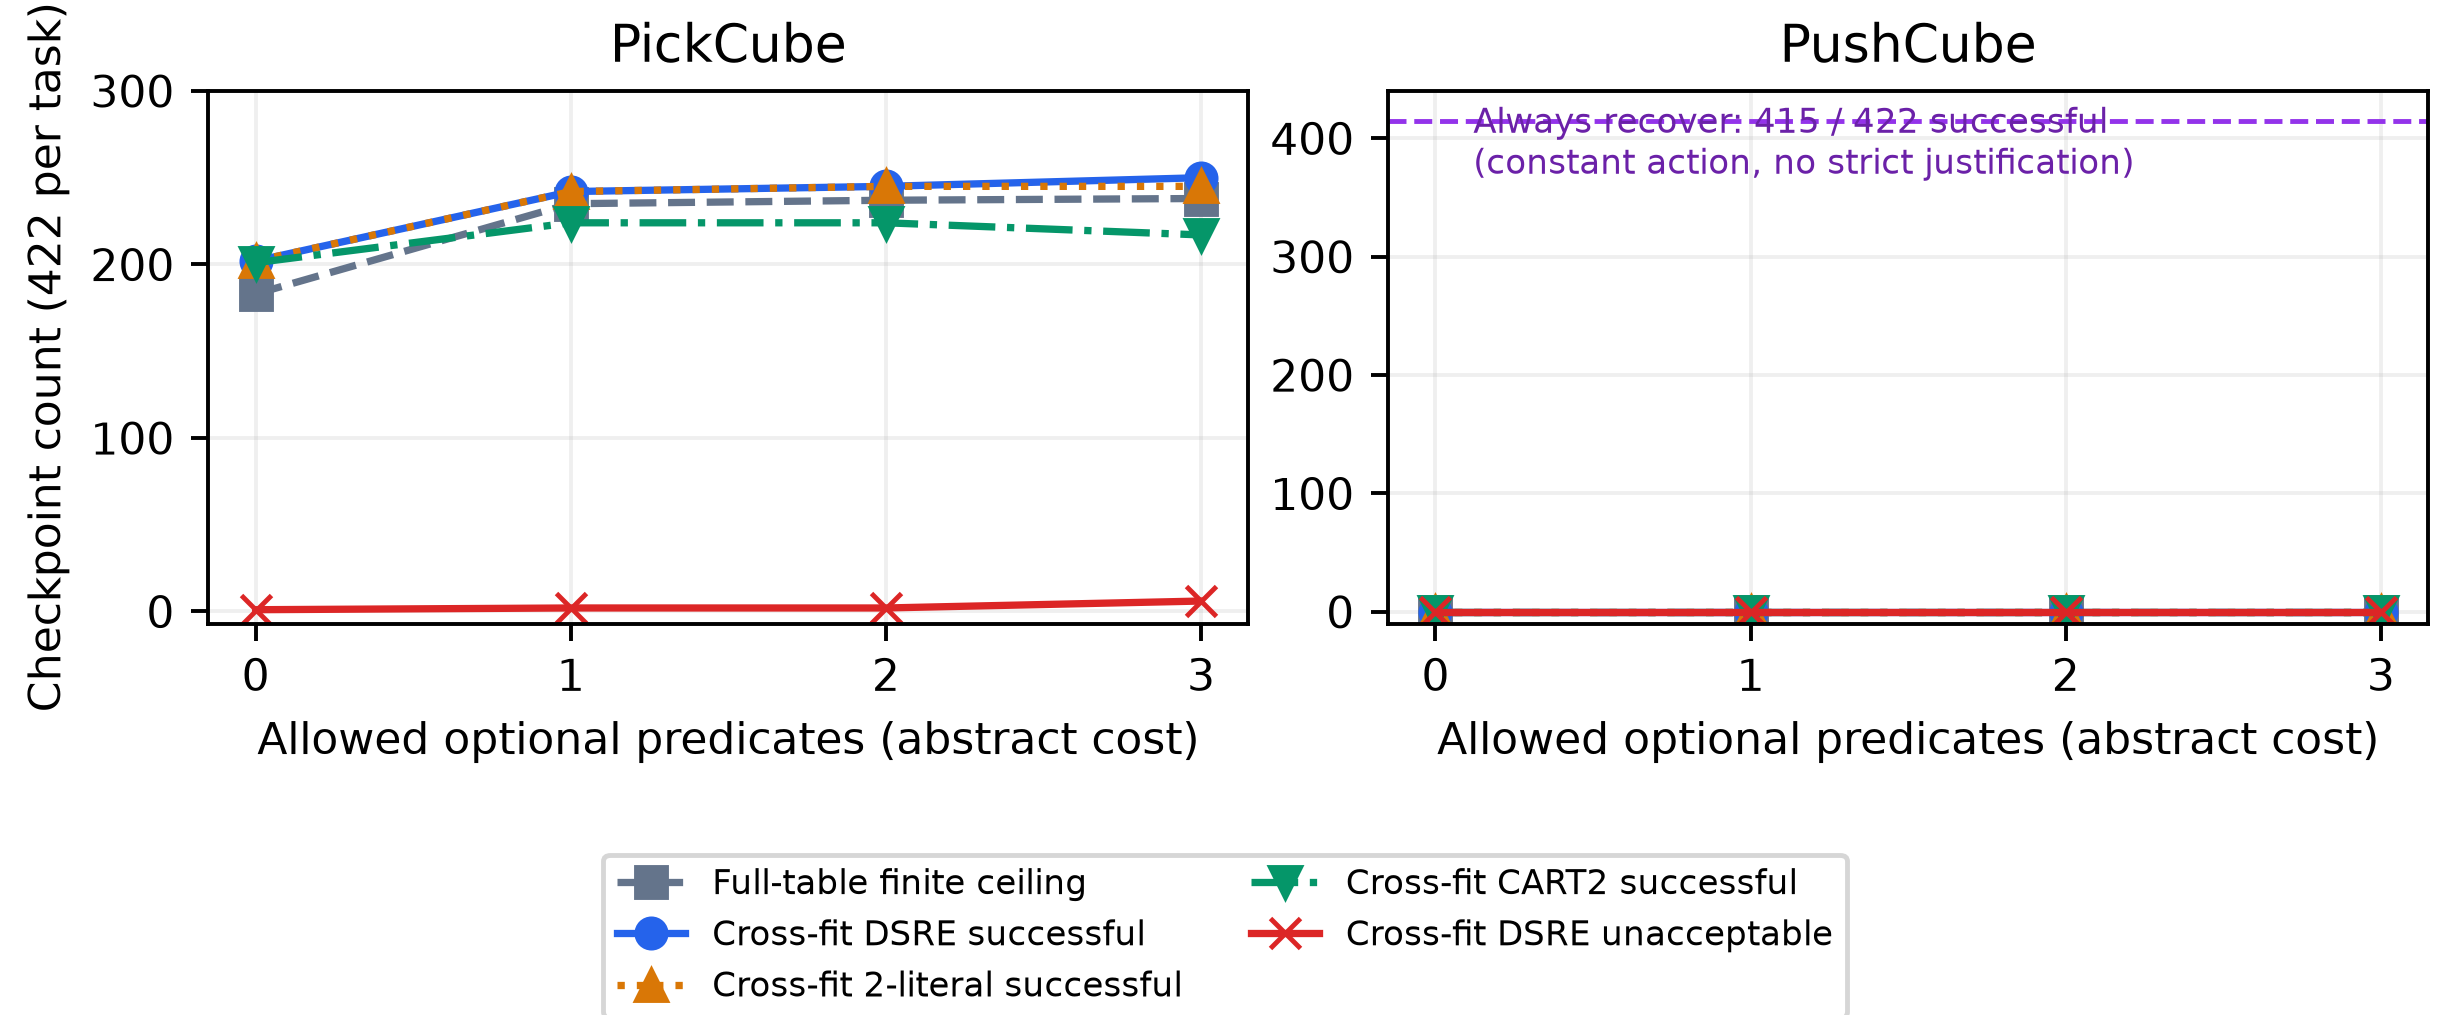
\includegraphics[width=\textwidth]{figures/frontier.png}
\caption{Finite-reference ceilings and exploratory grouped cross-fit outcomes are different estimands, each with 422 checkpoints/task. A cross-fit recommendation can exceed full-table actionable mass because its training reference omits conflicting held-out rows; that does not violate the refinement proposition. Cost counts optional Boolean pose predicates. PushCube strict curves coincide at zero. The two-literal control equals DSRE through b2; b3 gains include additional unacceptable choices.}
\label{fig:frontier}
\end{figure*}

\section{Hypotheses and Evaluation}
We test four fixed propositions: \textbf{H1}, added observable evidence increases finite strict justificability in some tasks; \textbf{H2}, sensing cannot make a neither-success checkpoint adequate; \textbf{H3}, finite strict coverage can differ sharply from high skill success; \textbf{H4}, held-out states can falsify extrapolation of finite-table sufficiency. H2 is structural; the others require empirical characterization. No hypothesis requires beating the equivalent B7 solver.

\subsection{Qualified reference and grouped reanalysis}
The experiments use ManiSkill3~\cite{maniskill} on a CPU backend. The reference has 844 qualified checkpoint pairs, 422 per task and 211 independent seed parents per task, after 76 exclusions from 920 candidate checkpoints. Each parent contributes two registered conditions: nominal/2-cm offset for PickCube and nominal/misaligned for PushCube. Both unchanged skills run for 70 controls, or 3.5 s, and adequacy uses terminal task success. Prefix replay and controller memory are qualified; native snapshots are not trusted for branching. Paired deterministic outcomes describe this simulator protocol, not repeated-trial success probabilities.

Six primary predicates summarize goal distance, hand--object distance, progress, object displacement, gripper closure and relative height. Six optional predicates test signed object--goal x/y offsets and hand--object x offsets against fixed $\pm.02$ m thresholds. All derive from simulator-supplied poses. They are observable interfaces in the experiment, not evidence for real visual perception or new sensing hardware. Privileged contact/grasp fields are diagnostic only and absent from primary queries.

We retain the original grouped five folds, holding both conditions of every seed together. Channel sets are selected on training parents only. All reference data have already informed development: this is exploratory cross-fitting, not untouched confirmation. We independently regenerate saved predictions, exact ceilings and error cases, and resample independent seed parents together for paired uncertainty. The paper reports counts and paired percentile intervals, not trajectory-row standard errors.

Equal-information controls include B7, one-/two-literal pure rules, outcome-aware CART depths 1--3, B5 at empirical error $.1$, a strict-first risk-aware wrapper, greedy coverage/entropy selectors, canonical/random menus and constant-action policies. Trees use four outcome classes and a shared two-parent inference gate. Controls that relax strictness are labeled provisional; their successes cannot be advertised as strict certificates.

\subsection{Frozen prospective check}
Before new outcomes, we fixed 200 unused seed parents per task, both registered conditions, b0 versus development-selected b1, full-development reference, support/ties, B5 and depth-1/2 CART comparators. Each outcome starts from a separate reset followed by the complete canonical action prefix. Every prefix state and controller memory must match before intervention; a fidelity/source failure stops the study without replacing seeds. New qualification checks checkpoint restoration, not duplicate future trajectories: the 1,600-continuation cap permits two actions per checkpoint, without additional future-rollout duplicates. Raw actions and terminal labels receive an independent offline audit.

Physics stops within three hours; incomplete parents are reported and excluded from primary paired inference. Four thousand paired parent-bootstrap draws estimate b1--b0 changes. The maximum 200 parents per task allows a worst-case normal 95\% half-width of 13.86 percentage points for bounded parent differences, so rare recovery assignments can remain underpowered. The study never samples until significance. Its frozen thresholds and reference are not updated with fresh outcomes. No deployment calibration is claimed.

\section{Results and Their Boundaries}


\begin{table}[t]
\caption{PickCube strict DSRE: reused grouped evaluation. Counts are recommendations / successful / unacceptable.}
\label{tab:main}\centering
\begin{tabular}{crrr}\toprule
Budget & Finite mass /422 & All starts /422 & Failed starts /145\\\midrule
0 & 183 & 203 / 202 / 1 & 19 / 19 / 0\\
1 & 235 & 244 / 242 / 2 & 19 / 18 / 1\\
2 & 237 & 247 / 245 / 2 & 22 / 21 / 1\\
3 & 238 & 256 / 250 / 6 & 31 / 26 / 5\\\bottomrule
\end{tabular}
\end{table}

\subsection{Finite gain, limited recovery evidence}
PickCube finite actionable mass rises from 183/422 with no optional predicates to 235, 237 and 238 at budgets one, two and three. All six yield 248, leaving 174 checkpoints outside a strict full-signature class. The first selected predicate is object-left-of-goal. PushCube remains zero at every budget, including all six channels; canonical minimum-cost selection therefore retains no optional predicate. These are exact statements about the fixed table, supporting H1 selectively and H2 structurally, rather than bounds on unseen states.

Cross-fit PickCube successful strict recommendations rise from 202 to 242 with b1: $+9.48$ percentage points, independently regenerated paired 95\% interval $[6.64,12.32]$. But recommendations include one versus two unacceptable choices, so ``strict'' describes reference purity and not zero held-out error. The b1 gain is concentrated in 277 initially successful starts. In the 145 initially failed starts, successful recommendations fall from 19 to 18, with one unacceptable action. At b3 this subset reaches 26 successes but five unacceptable choices. Thus the overall frontier does not establish improved physical failure recovery. Increased success-maintenance coverage may be useful, but requires a different deployment argument.

\subsection{Strong controls and counterexamples}
B7 agrees with DSRE in all 16,880 registered views. Two-literal pure rules agree through b2; at b3 they recommend 248 times with three unacceptable choices, versus 256 with six for DSRE. Depth-2 strict CART gives 202, 225, 225 and 218 successful recommendations with one unacceptable choice at each budget. Exact and greedy coverage selection coincide at b1. At b3 exact selection adds eight successes over greedy coverage, but also four unacceptable choices and one predicate; this is not a free improvement or a new optimization principle.

Provisional criteria can yield more actions. For PickCube, depth-2 CART at $.9$ empirical purity gives 297 successes and one unacceptable choice at b0, compared with strict DSRE's 202 and one; the comparison changes the justification standard. For PushCube, always recovering succeeds in 415/422 checkpoints, including five neither-success states and two continue-only states among its seven failures. Strict coverage nevertheless remains zero: compatible classes retain unfavorable outcomes, including six unseparable opposing-action edges under the entire menu. High skill success and strict observable justification therefore differ sharply, supporting H3 without claiming the recovery skill is ineffective.

The strict held-out errors arise when training-pure conjunctions meet unseen adverse outcomes, including neither-success checkpoints. They are direct evidence for H4. More predicates can isolate sparse classes while leaving the finite reference fragile. Witnesses explain the reference obstruction and minimum rule, but do not certify that the reference exhausts the future population. We retain all failures and do not relabel neither-success cases as harmless abstentions.

\subsection{Prospective evidence: incomplete cohort, unchanged failure recovery}
The worker exited with SIGTERM before the planned cohort finished; its cause is not established by retained evidence. The registered runtime-failure stop was followed without relaunch or replacement. We retain 133 qualified checkpoints: 132 from 66 complete parents (33/task) and one orphan condition, excluded from primary inference. Of 800 planned checkpoints, 667 lack qualified paired outcomes. These are genuinely new, frozen-reference measurements, but only an incomplete fixed-order subset, not completion of the 400-parent confirmation. Interruption-related selection bias cannot be ruled out.

\begin{table}[t]
\caption{Prospective complete-parent subset. Strict DSRE counts are recommendations / successful / unacceptable. Strict CART2 matches every decision in these rows.}
\label{tab:fresh}\centering
\begin{tabular}{lcrr}\toprule
Task & $b$ & All starts /66 & Failed-start good / starts\\\midrule
Pick & 0 & 29 / 29 / 0 & 6 / 20\\
Pick & 1 & 38 / 38 / 0 & 6 / 20\\
Push & 0 & 0 / 0 / 0 & 0 / 66\\
Push & 1 & 0 / 0 / 0 & 0 / 66\\\bottomrule
\end{tabular}
\end{table}

PickCube b1 adds nine successful strict recommendations: $+13.64$ percentage points, paired parent-bootstrap 95\% interval $[6.06,21.21]$. All nine occur among 46 initially successful starts. The 20 initially unsuccessful starts retain the same six successes, five assigned recover and one continue. There are zero observed strict errors at either budget, but only five independent parents receive recovery. This is neither evidence of zero population error nor the required independent calibration. PushCube still abstains on every checkpoint, although recovery succeeds in all 66 fresh cases; its frozen reference retains incompatible outcomes.

The strongest controls prevent a method-advantage interpretation. Strict depth-2 CART matches all 264 task/checkpoint/budget decisions, including abstentions; B7 also matches minimum explanations. At b1, DSRE uses 52 literals across 38 Pick recommendations versus 76 for the tree, but the ordinary exact rule has the same brevity. This is not a measured human benefit. Provisional $.9$ CART succeeds in 53/66 Pick checkpoints with no observed errors (7/20 failed starts), at both budgets. DSRE's b1 success coverage is lower by 22.73 percentage points, paired 95\% interval $[-30.34,-13.64]$. Ordinary B5 instead succeeds in 48/66 with five unacceptable choices. These methods change the strict justification standard; still, their observed performance makes a broad utility advantage untenable.

An independent recorded-physics audit checks all 133 traces, 18,962 prefix states and 18,620 intervention controls. Controller actions rederived from pre-action packets agree exactly. Independent rule enumeration, direct frozen-tree leaf evaluation, and literal/obstruction checks verify 2,640 prediction views. This is separate implementation within the same session, not external human replication. Checkpoint restoration is qualified; future trajectories were not independently duplicated. No safety or calibration claim follows from this subset.

\section{Discussion and Stage 2 Questions}
The evidence supports a modest, falsifiable characterization. Representation refinement can improve finite justificability, yet its observed held-out gains need not occur where recovery is needed. A highly effective skill may remain unjustifiable under a coarse predicate vocabulary. Exact sufficient explanations expose these boundaries but are neither an improved controller nor a population safety guarantee. The strongest baseline equivalence is expected and should constrain any claim of novelty.

Several limitations are substantive. There are only two simulated tasks, two fixed interventions and binary horizon-dependent utility. The deterministic paired labels do not measure stochastic repeatability, hardware robustness or human usefulness. Optional channels reuse idealized poses; their unit cost is representational, not sensor expenditure. Development cohorts and rare recovery-support classes are small. The primary menu does not vary enough in PushCube; a zero ceiling is conditional on that menu. Cross-fitting reuses data that shaped the research, and no conformal or risk-control guarantee follows from purity or the two-parent gate. Calibration and executable action permission remain disabled.

The fresh subset reinforces the all-start observation effect but offers no failed-start gain or advantage over the strict tree. Completing a separately authorized, prospectively fixed study would address precision and interruption-related missingness, not resolve the known algorithmic equivalence. Stage 2, if invited, should test independent calibration under stated sampling assumptions, richer but prospectively frozen observations with actual sensing cost, stochastic repeatability, and transfer beyond the two tasks. None is an accomplished result here. A useful contribution must show that the witness/frontier formulation changes a robotics decision beyond what a simple known rule interface already provides; packaging alone does not establish this. We therefore present DSRE as a transparent empirical methodology with unresolved distinctiveness, not a new universally superior explanation algorithm.

\clearpage
\bibliographystyle{plainnat}
\bibliography{references}
\end{document}
